\documentclass[]{standalone}
\usepackage[dvipsnames]{xcolor}
\usepackage{tikz-network}
\begin{document}
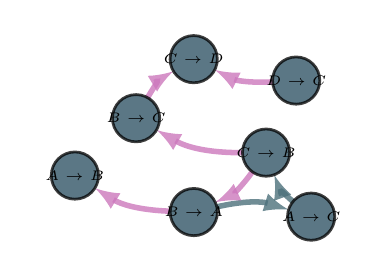
\begin{tikzpicture}
    \pgfmathsetmacro{\width}{3.0}
    \pgfmathsetmacro{\height}{2.0}
    \pgfmathsetmacro{\margin}{0.5 + 0.2}
    \tikzset{every node}=[font=\sffamily\bfseries]
    \clip (-\margin*\width cm,-\margin*\height cm) rectangle (\margin*\width cm,\margin*\height cm);
    \draw[draw,opacity=0] (-\margin*\width cm,-\margin*\height cm) rectangle (\margin*\width cm,\margin*\height cm);
    \Vertex[label=$A\to B$,fontsize=\fontsize{4}{10}\selectfont,RGB,color={36, 74, 92},size=0.6,opacity=0.75,style={draw opacity=0.75},x=-1.5,y=-0.47825933]{A->B};
\Vertex[label=$A\to C$,fontsize=\fontsize{4}{10}\selectfont,RGB,color={36, 74, 92},size=0.6,opacity=0.75,style={draw opacity=0.75},x=1.5,y=-1.0]{A->C};
\Vertex[label=$B\to A$,fontsize=\fontsize{4}{10}\selectfont,RGB,color={36, 74, 92},size=0.6,opacity=0.75,style={draw opacity=0.75},x=0.00982064,y=-0.9417213]{B->A};
\Vertex[label=$B\to C$,fontsize=\fontsize{4}{10}\selectfont,RGB,color={36, 74, 92},size=0.6,opacity=0.75,style={draw opacity=0.75},x=-0.7233619,y=0.25018406]{B->C};
\Vertex[label=$C\to B$,fontsize=\fontsize{4}{10}\selectfont,RGB,color={36, 74, 92},size=0.6,opacity=0.75,style={draw opacity=0.75},x=0.9278133,y=-0.18667328]{C->B};
\Vertex[label=$C\to D$,fontsize=\fontsize{4}{10}\selectfont,RGB,color={36, 74, 92},size=0.6,opacity=0.75,style={draw opacity=0.75},x=0.008578956,y=1.0]{C->D};
\Vertex[label=$D\to C$,fontsize=\fontsize{4}{10}\selectfont,RGB,color={36, 74, 92},size=0.6,opacity=0.75,style={draw opacity=0.75},x=1.3098919,y=0.72834086]{D->C};
\Edge[bend=15,Direct,RGB,color={76, 112, 123},lw=2,opacity=0.8](A->C)(C->B);
\Edge[bend=15,Direct,RGB,color={204, 120, 188},lw=2,opacity=0.8](B->A)(A->B);
\Edge[bend=15,Direct,RGB,color={76, 112, 123},lw=2,opacity=0.8](B->A)(A->C);
\Edge[bend=15,Direct,RGB,color={204, 120, 188},lw=2,opacity=0.8](B->C)(C->D);
\Edge[bend=15,Direct,RGB,color={204, 120, 188},lw=2,opacity=0.8](C->B)(B->A);
\Edge[bend=15,Direct,RGB,color={204, 120, 188},lw=2,opacity=0.8](C->B)(B->C);
\Edge[bend=15,Direct,RGB,color={204, 120, 188},lw=2,opacity=0.8](D->C)(C->D);

\end{tikzpicture}
\end{document}
